\documentclass[svgnames]{beamer}

\usetheme{Madrid}
\usecolortheme{seahorse}
\usepackage{multirow}
\usepackage{caption}
\setbeamertemplate{navigation symbols}{}
\useinnertheme{rectangles}

\usepackage{appendixnumberbeamer}
\usepackage[ruled, vlined, longend]{algorithm2e}

\beamertemplatenavigationsymbolsempty
\usepackage[many]{tcolorbox}
\usepackage{color}
\usepackage{varwidth}
\usetikzlibrary{decorations.pathmorphing}
\usetikzlibrary{shadows}
\usetikzlibrary{svg.path}
\usepackage[absolute,overlay]{textpos}

\usepackage{listings}
\lstset {
  backgroundcolor=\color{white},
  basicstyle=\ttfamily\footnotesize,
  numbers=left,numberstyle=\tiny,numbersep=5pt,
  emph={proc, fun, let, send, consume, global, type, record, if, else,
    in, not, foldt, return, on, ordering, by, as, or },
  emphstyle={\bfseries},
  literate = {=>}{{\bf=>}}2
}
\usepackage{graphicx,accents,pinlabel}
%\useoutertheme{default}
%\useinnertheme{rounded}

\titlegraphic{
\begin{center}
\includegraphics[width=6cm]{poker_routes}%
\end{center}
}

\usepackage{tikz}
\usetikzlibrary{fadings,shapes.arrows,shadows}
\usetikzlibrary{shadows.blur}
\usetikzlibrary{shapes.symbols}
\usetikzlibrary{backgrounds}
\usetikzlibrary{arrows.meta}
\usetikzlibrary{shapes,snakes}
\usetikzlibrary{fit,calc,shadows}
\usetikzlibrary{arrows,shapes}
\setbeamercolor{section in head/foot}{bg=white, fg=black}
%\beamertemplateshadingbackground{black!10}{blue!15}
\makeatletter
\setbeamertemplate{footline}
{
  \leavevmode%
  \hbox{%
  \begin{beamercolorbox}[wd=.333333\paperwidth,ht=2.25ex,dp=1ex,center]{section in head/foot}%
    \usebeamerfont{author in head/foot}\insertshortauthor~~\beamer@ifempty{\insertshortinstitute}{}{}
  \end{beamercolorbox}%
  \begin{beamercolorbox}[wd=.333333\paperwidth,ht=2.25ex,dp=1ex,center]{section in head/foot}%
    \usebeamerfont{date in head/foot}\insertshortdate{}\hspace*{2em}
  \end{beamercolorbox}%
  \begin{beamercolorbox}[wd=.333333\paperwidth,ht=2.25ex,dp=1ex,right]{section in head/foot}%

    \insertframenumber{} / \inserttotalframenumber\hspace*{2ex} 
  \end{beamercolorbox}}%
  \vskip0pt%
}
\makeatother
\title{Mixed and time varying models for evolving complex networks}
\titlegraphic{
\begin{center}
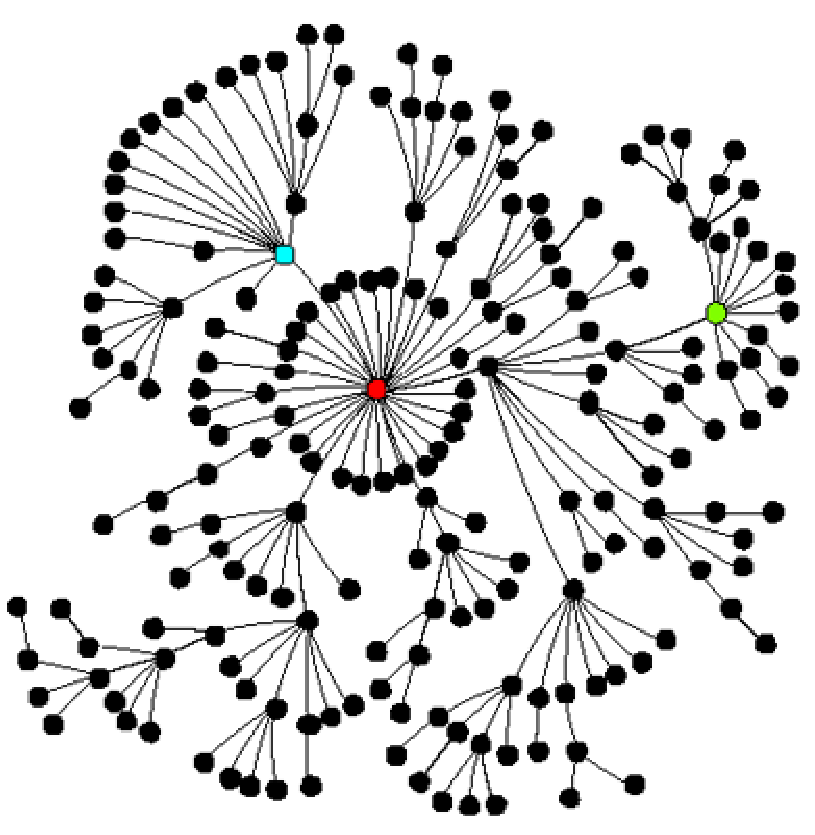
\includegraphics[width=3cm]{scale1}%
\end{center}
}

\author[Richard G. Clegg \& Naomi Arnold] {Richard G. Clegg (r.clegg@qmul.ac.uk) \\ 
Naomi Arnold (n.a.arnold@qmul.ac.uk) \\
Queen Mary University of London } 

\newcommand{\mr}{\mathbb{R}} %math R%
\newcommand{\mn}{\mathbb{N}} %math N%
\newcommand{\mz}{\mathbb{Z}} %math Z%
\newcommand{\bG}{\mathbf{G}}
\newcommand{\bg}{\mathbf{g}}
\newcommand{\btheta}{\mathbf{\theta}}
\newcommand{\var}[1]{\text{var}\left(#1\right)}
\newcommand{\Esym}{\text{E}}
\newcommand{\E}[1]{\Esym\left[#1\right]}
\newcommand{\Probsym}{\mathbb{P}}
\newcommand{\Prob}[1]{\Probsym\left[#1\right]}
\definecolor{burntorange}{cmyk}{0,0.52,1,0}
\tikzstyle{superpeers}=[draw,circle,burntorange, left color=\oran,
                       text=violet,minimum width=20pt]

\tikzstyle{big comment} = [draw, fill=blue!40, text=white, text width=8cm, minimum height=0.8cm, rounded corners, drop shadow, align=center]
\def\oran{orange!30}
\tikzstyle{vertex}=[circle,fill=black!25,minimum size=20pt,inner sep=0pt]
\tikzstyle{edge} = [draw,ultra thick,-]

\date[NetSci 3, Leeds]{3rd UK Network Science Workshop, Leeds 2019}

\begin{document}

\frame{

\begin{center}
\Huge{\inserttitle}


\vspace{0.2cm}

\inserttitlegraphic

\vspace{0.2cm}

\scriptsize{\insertauthor}

\vspace{0.2cm}

\scriptsize{\insertdate}

\vspace{0.2cm}

\tiny{(Prepared using \LaTeX \;and beamer.)}
\end{center}
}


\frame{
\frametitle{Problem statement}
\begin{itemize}
\item Evolving networks (graphs/topologies) 
are an important topic for research.
\item Want to describe and understand processes which govern
evolution.
\item Motivating example models of similar form to Barab\'asi--Albert (1999)
\end{itemize}
\begin{block}{Problem statement (vague)}
\begin{itemize}
\item Want to grow networks with the \alert{same properties} as
real networks.
\item Want to be able to describe the \alert{evolution} 
of the real network.
\item Want to be able to compare rival theories about the evolution.
\end{itemize}
\end{block}
}
\tikzstyle{edge} = [draw,ultra thick,-]

\frame{
\frametitle{Many many network models exist}

\begin{itemize}
\item Degree to power model [Krapivsky et al Phys Rev Lett 2000] 
\begin{itemize}
\item Probability of attachment to $i$ is degree $d_i$ modified by power $p_i \sim  d_i^ {\alpha}$ -- $\alpha$ is tunable parameter.
\end{itemize}
\item Positive Feedback Preference (PFP model) [Zhou--Mondrag\'on Phys Rev E 2004] (targetted at the Internet)
\begin{itemize}
\item Prob. of connecting to $i$ is 
$p_i \sim 
d_i^ {(1 - \delta \log_{10} d_i)}$ where
$\delta$ is a tunable parameter.
\end{itemize}
\item Jackson--Rogers [American Econ Rev 2007] (targetted at social networks)
\begin{itemize}
\item (Simplified explanation).  Pick $r$ nodes completely at random.  Pick $q$ nodes that neighbour these $r$ nodes.  $q$ and $r$ are tunable parameters.
\end{itemize}
\item Many others: Stochastic block models, exponential random graphs, Waxman model, Subgraph generation model, Statistical exponential random graphs.
\end{itemize}
}

\subsection{Problems arising}

\frame{
\frametitle{The ``basket of statistics" approach}



\begin{itemize}
\item Which model is ``best"?  How do we tune parameters?
\item Define the current approach the ``basket of statistics" method.
\begin{enumerate}
\item Select several statistics which can be measured on net snapshot.
\item Use test model to grow test network (same size as real network).
\item Compare the ``basket of statistics" on real and test.
\end{enumerate}
\item New statistics motivate new models -- but what if not all stats match?
\end{itemize}

Topology modelling appears to be progressing in the following manner:
\begin{enumerate}
\item Analyse snapshot of graph (topology) of interest.
\item Find some statistic  the current
model does not replicate (add this to ``basket").
\item Create a new model which replicates the new statistic without
affecting old ones.
\item Test using the above procedure. 
\end{enumerate}

}


\frame{
\frametitle{Refined problem statement}
\begin{itemize}
\item Let $G(t)$ be a time evolving graph which evolves according
to some probabilistic process.
\item Let $\bG= (G_i, G_{i+1}, \ldots, G_{i+n})$ be random variables
representing this process observed at discrete times.
\item Let $\bg=(g_i, g_{i+1}, \ldots, g_{i+n})$ be a set of observations
of $\bG$.
\end{itemize}
\begin{block}{Problem statement --- more precise}
Given observations of a graph $\bg$ want to:
\begin{itemize}
\item Create models which formally specifies $\Prob{G_{t+1} = g_{t+1} | 
G_t=g_t,\ldots}$.
\item Likelihood is a term in statistics it measures the probability a given data set arose if an explanatory model is true.
\item Measure the likelihood of such a model producing $\bg$.
\item Automatically test many such models.
\end{itemize}
\end{block}
}

\section{FETA}

\subsection{FETA approach}
\frame{
\frametitle{FETA approach}


\begin{block}{FETA}
Framework for Evolving Topology Analysis
\end{block}

\begin{center}
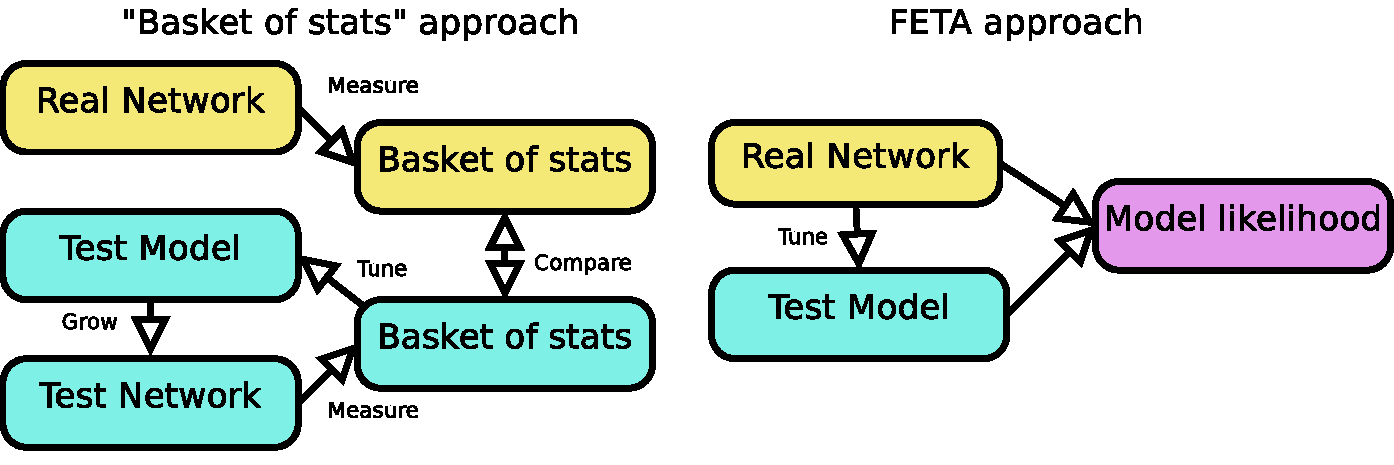
\includegraphics[width=10cm]{feta_process}
\end{center}
}

\subsection{A probabilistic model of graph evolution}
\frame{
\frametitle{A probabilistic model of graph evolution}
\begin{itemize}
\item Creating a parameterised model $M(\btheta)$ of $\Prob{G_{t+1} = g_{t+1} | 
G_t=g_t,\ldots}$.
is not straightforward.
\item This is not like normal stochastic process.  The dimensionality
of $G(t)$ changes over time.
\item Could transform to some multi-dimensional process with
dimension highest dimension graph will achieve (nasty solution).
\item Also want a solution which is compatible with existing research
in field (can test existing research methods).
\end{itemize}
}


\frame{
\frametitle{The FETA model structure}
\begin{block}{Operation model}
\begin{itemize}
\item Process to select an operation on the network.
\item Could be: \alert{add node}, 
\alert{add edge}, 
\alert{remove node} and so on.
\end{itemize}
\end{block}

\begin{block}{Object model}
\begin{itemize}
\item Process selects which nodes/edges are involved in operation
selected by operation model.
\item Probabilities are assigned to nodes and potential
edges for random selection.
\item Edges selected by assigning probabilities
to node pairs.
\item Object model is main focus of this presentation (operation model, for now ``copied").
\end{itemize}
\end{block}
}

\subsection{Object Model evaluation}


\subsection{From model to likelihood}

\frame{
\frametitle{The likelihood of FETA model}
\begin{itemize}
\item Let $M(\btheta)$ be a parameterised FETA model which
assigns probabilities to operations and object models with
some parameters $\btheta$.
\item Define $f_{i,M(\btheta)}(g_i)= \Prob{G_{i}=g_i| M(\btheta), G_{i-1}=g_{i-1}, 
G_{i-2}=g_{i-2}, \ldots}$
\item For convenience just write  $f_{i}(g_i)$
\item Then the likelihood of the model $M(\btheta)$ given the
observations $\bg$ (from $i$ to $i+n$)
is
$L(M(\btheta) | \bg ) = \prod_{k=i+1}^{k=i+n} f_k(g_k)$.
\item This likelihood defines how likely the model is given
the observations (or conversely, how probable the observations given
the model).
\item It is the ability to assign a true likelihood to the
graph evolution which is key to the FETA process.
\end{itemize}
}

\frame{
\frametitle{Insight: we can build models from components}
\begin{block}{Unlikely that any one model is the ``whole" truth}
Can we create new models by ``mixing" existing model components? \\
Take two (or more) models and create a model that mixes both in some proportion.
\end{block}
\begin{itemize}
\item How about mixture models?  
\item We can mix an arbitrary number of models.  Let $p_i^{(n)}$ be the 
probability of choosing node $i$ in model $n$
$$
p_i = \beta_1 p_i^{(1)} + \beta_2 p_i^{(2)} + \cdots
$$
where $0 \leq \beta_i \leq 1$ and $\sum_i \beta_i = 1$.
\end{itemize}
}

\frame{
\frametitle{Object model components}
Throughout $k$ is a normalising constant such that $\sum_i p_i = 1$
for all nodes considered.  
$p_i$ is the probability of picking node
$i$ (at the stage being considered).

\begin{itemize}
\item Random model $M_0 \quad p_i = 1/k$.
\item Preferential attachment $M_d \quad p_i = d_i /k$.
\item PFP $M_p(\delta) \quad p_i = d_i^{1+\delta \log_{10} (d_i)}/k$  where $\delta$ is a parameter.
\item Degree power $M_d(\alpha) \quad p_i = d_i^{\alpha}/k$ where $\alpha$ is a parameter.
\item Triangle model $M_t(N) = 1/k$ if node in neighbourhood of $N$ most recently chosen. 
\end{itemize}
}


\section {Testing FETA}

\subsection{Artificial tests}

\frame{
\frametitle{Artificial tests}
\begin{itemize}
\item Perhaps the most convincing test of such a model is its ability to
recover parameters from a known model.
\item Create a realisation of a graph with known $M(\btheta)$.  
\item From this graph try to recover $\btheta$ with maximum likelihood.
\item Linear parameters of model can be assessed ``in parallel" (model tracks likelihood for a range of answers simultaneously).
\item Other (non-linear) parameters can be found from ``parameter sweeps" 
(assessing the likelihood for many values of that parameter).
\item Look at a measure $c_0$ which gives a ``human readable" likelihood relative to a null model of ``random" connections.
\end{itemize}
}

\frame{
\frametitle{Sweep one parameter (10,000 link network)}
\centering{
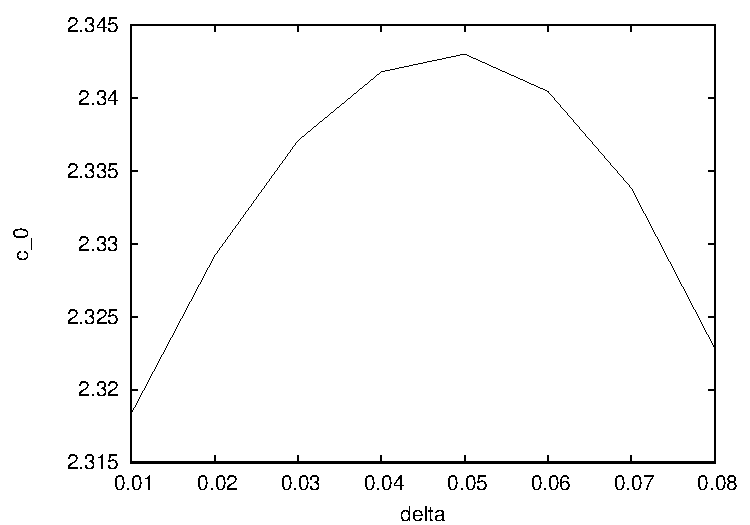
\includegraphics[width=10cm]{deltasweep} \\
}
PFP model $M= M_d(0.05)$.  Correct answer is $\delta = 0.05$.
}

\frame{
\frametitle{Sweep two parameters (10,000 link network)}
\centering{
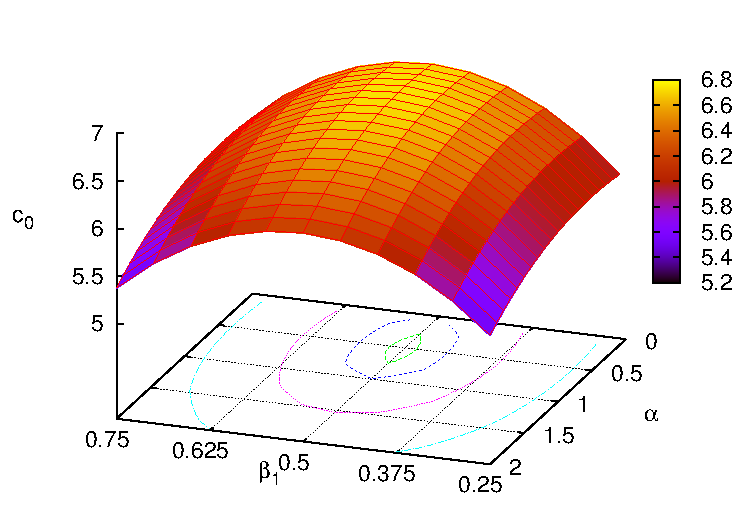
\includegraphics[width=8cm]{art1_data} \\
}
Correct model $M = 0.5 M_2 + 0.5 M_d(0.5)$
fitted $M= \beta_1 M_2 + (1-\beta_1) M_d(\alpha)$.
}


\subsection{Real tests}

\frame{
\frametitle{Real tests FB data (1)}
\begin{center}
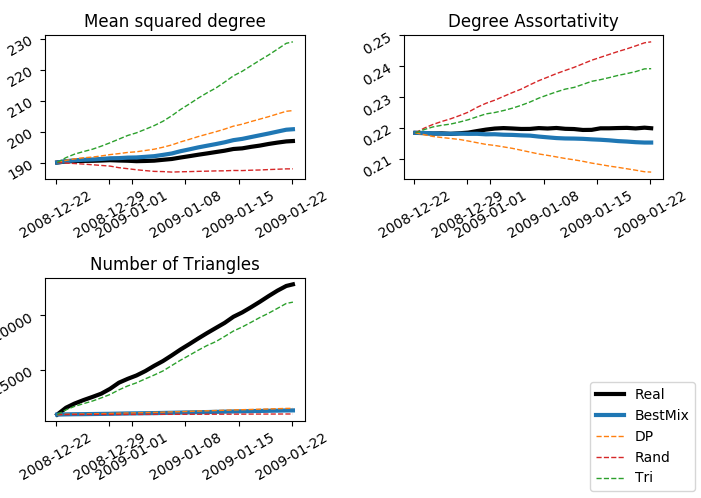
\includegraphics[width=0.9\textwidth]{FBright}
\end{center}
}

\frame{
\frametitle{Real tests FB data (2)}
\begin{center}
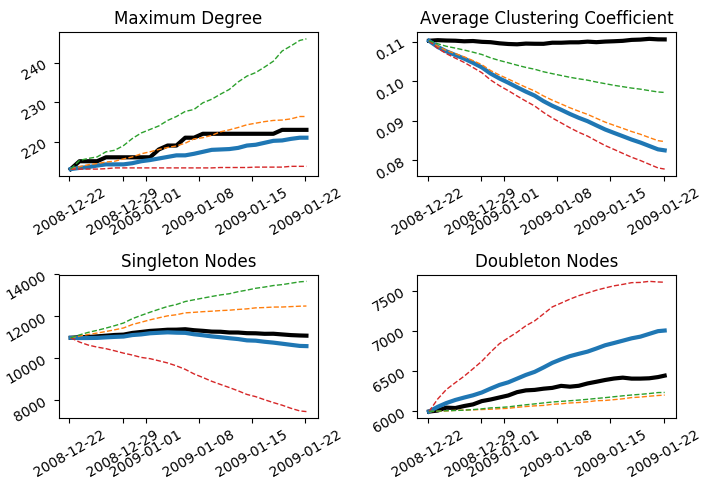
\includegraphics[width=0.9\textwidth]{FBleft}
\end{center}
}

\frame{
\frametitle{Summary so far}
\begin{itemize}
\item FETA can give an exact likelihood a model $M$ underlies an observed dynamic graph.
\item Given several models and a data set FETA can say which is the most likely to have produced that data.
\item FETA can take several models and produce a ``mixture" of all three.
\item On artificial data sets produced from mixture models FETA can recover the parameters.
\item On real data we can test mixtures of models improving replicated statistics.
\item Next step, what if underlying model changes during lifetime of graph.  
\end{itemize}
}

\section{Models which change in time}

\frame{
\frametitle{Models which change in time}
\begin{itemize}
\item{Motivating examples}
\begin{itemize}
\item A social network which changes its rules (default privacy assumptions, maximum number of followers).  
\item A network associated with an organisation suffers a traumatic event (enron email network).
\item A network associated with a technological change (bitcoin network when chain forks, Internet as technology evolves).
\end{itemize}
\item In this case it is likely the underlying model will change as time changes.
\item How can we model this?
\end{itemize}
}


\frame{
\frametitle{Models which change in time -- artificial data}
\begin{itemize}
\item Model changes once at time $T$.  Use the ``degree power" model and change the power.
\item Let $p_i(t)$ be the probability of choosing $i$ at time $t$.
\item Let $d_i(t)$ be the degree of $i$ at time $t$.
$$p_i(t) =
\begin{cases} d_i(t)^\alpha/k & t < T \\
d_i(t)^\beta/k & t \geq T.
\end{cases} 
$$
\item Now we can grow a graph using this model for different $\alpha$ and $\beta$.
\item Already shown for a long section of data we can recover the parameter.
\item Can we locate the point at which the change occurs?
\end{itemize}
}

\subsection{Finding the change point}

\frame{
\frametitle{Finding the change point -- 10000 node experiment}
\begin{center}
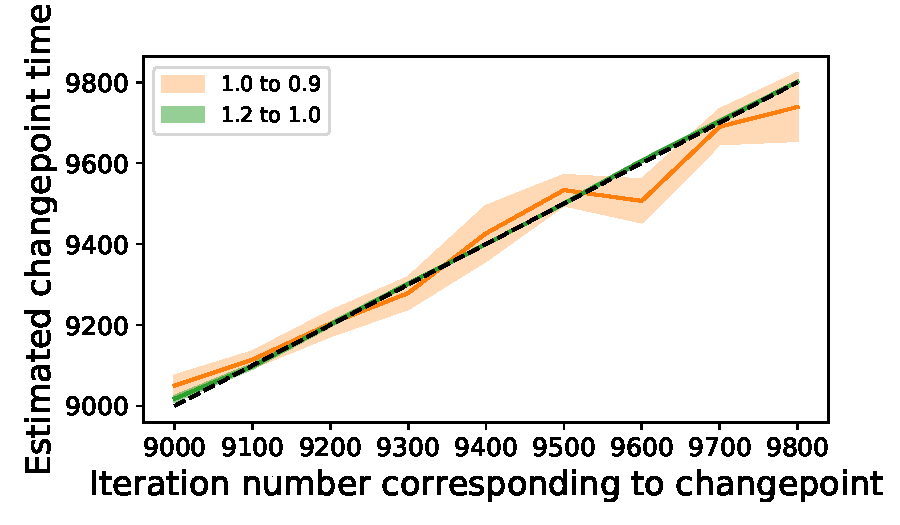
\includegraphics[width=0.9\textwidth]{DP10000_diff_markers}
\end{center}
}


\frame{
\frametitle{Finding the change point -- 1000 node experiment}
\begin{center}
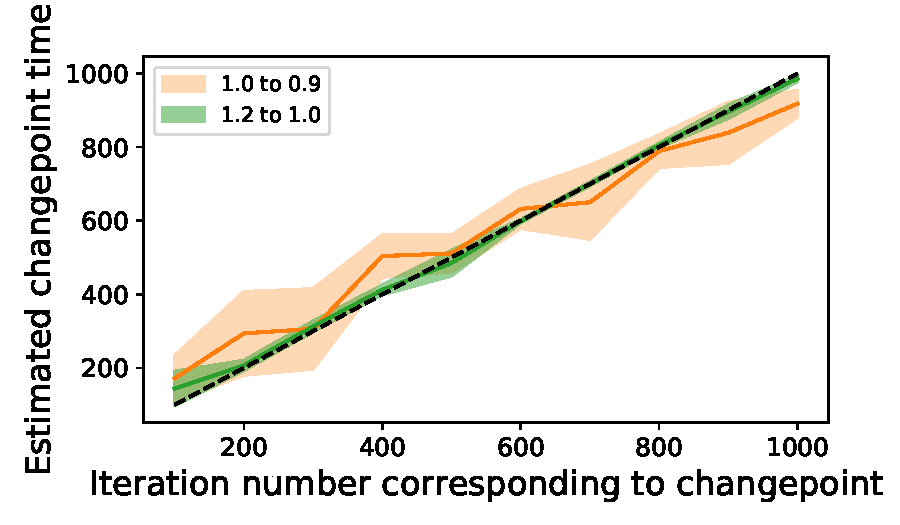
\includegraphics[width=0.9\textwidth]{DP1000_diff_markers}
\end{center}
}


\frame{
\frametitle{Which changes are easiest to detect?}
\begin{center}
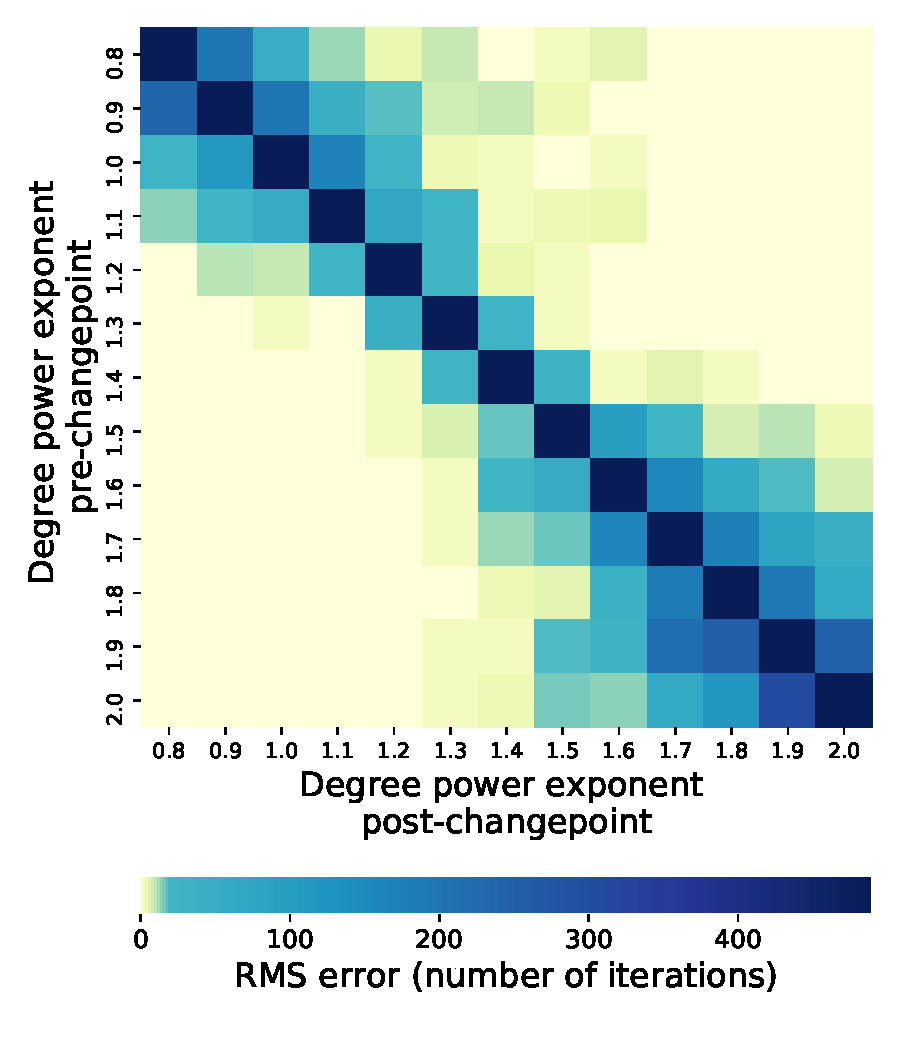
\includegraphics[width=0.9\textwidth]{DP_rescaled_heatplot}
\end{center}
}

%\frame{
%\frametitle{Sweep two parameters (10,000 link network)}
%\begin{center}
%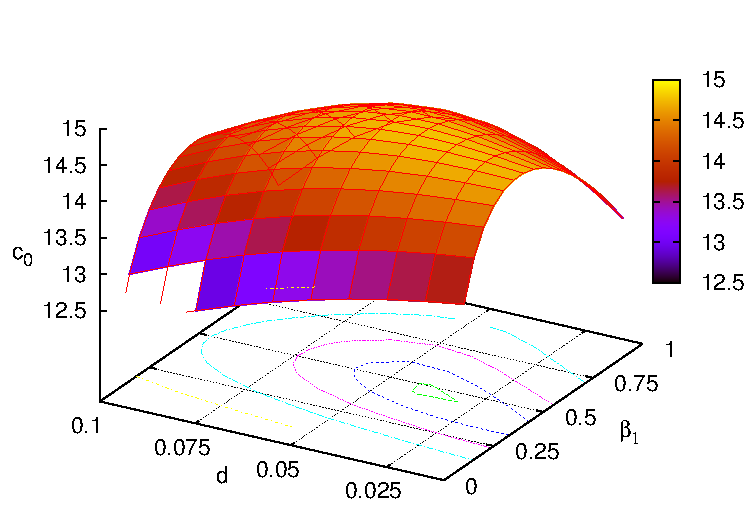
\includegraphics[width=8cm]{art2_data} \\
%Correct model $M = 0.5M_p(0.05)+0.5M_t$ fitted 
%$M= \beta_1 M_p(d)+(1- \beta_1)M_t$ 
%\end{center}
%}


\tikzstyle{big comment} = [text=white, minimum height=0.8cm, rounded corners, align=center]

\frame{
\frametitle{Changes in real data -- Enron email network analysed as 3 model mixture 10 time periods}
\centering{
\begin{tikzpicture}%[show background grid]
\node<1-> at (0,0){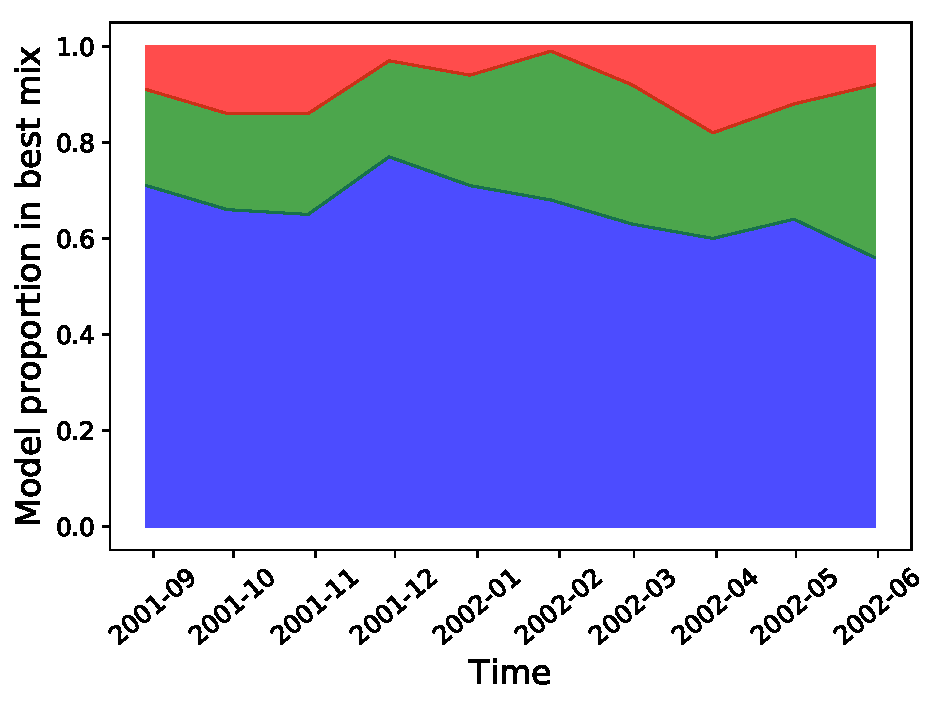
\includegraphics[width=0.85\textwidth]{EnronMixtures}};
\node<1->[big comment] at (-3,1.3){BA};
\node<1->[big comment] at (-3,2.2){Tri};
\node<1->[big comment] at (-3,3){Rand};
\draw<2-> [dashed, white, thick] (-0.9,3.2) -- (-0.9,-2.5);
\node<2->[big comment] at (-0.9,0){Enron files\\for bankrupcy};
\draw<3-> [dashed, white, thick] (2.6,3.2) -- (2.6,-2.5);
\node<3->[big comment] at (2.6,0){Obstruction charge\\for destroying files};
\end{tikzpicture}
}
}

\section{Conclusions}
\subsection{Conclusions}

\frame{
\frametitle{Conclusions}
\begin{itemize}
\item The likelihood parameters and the null model here provide 
a rigorous way to assess a potential dynamic model of network evolution.
\item The advantages of this framework are several:
\begin{enumerate}
\item Assesses the dynamic history of the data not statistics of
a snapshot.
\item Single statistically rigorous estimate of model
likelihood.
\item Quicker than growing a network and testing
statistics.
\item Models can be mixture and vary in time.
\end{enumerate}
\item An exciting new way to test theories about topologies
if you have the data for it.
\end{itemize}
}

\frame{
\frametitle{Further work}
\begin{itemize}
\item Ongoing work -- lots still to do.
\item Software and data freely available -- please email 
{\tt n.a.arnold@qmul.ac.uk}
\item Code and data: 
{\tt https://github.com/narnolddd/FETA3}
\end{itemize}
}



\end{document}
